\documentclass[margin=1cm]{standalone}

\usepackage{tikz}
\usetikzlibrary{arrows, fit, positioning, calc}
\usetikzlibrary{arrows.meta}
\usetikzlibrary{decorations.text}
\usetikzlibrary{decorations.pathmorphing}

\newcommand{\hole}[2]{%
    \draw (#1) circle (#2);
    \draw ($(#1) - (#2, 0)$) -- ($(#1) + (#2, 0)$);
    \draw ($(#1) - (0, #2)$) -- ($(#1) + (0, #2)$);
}

\begin{document}
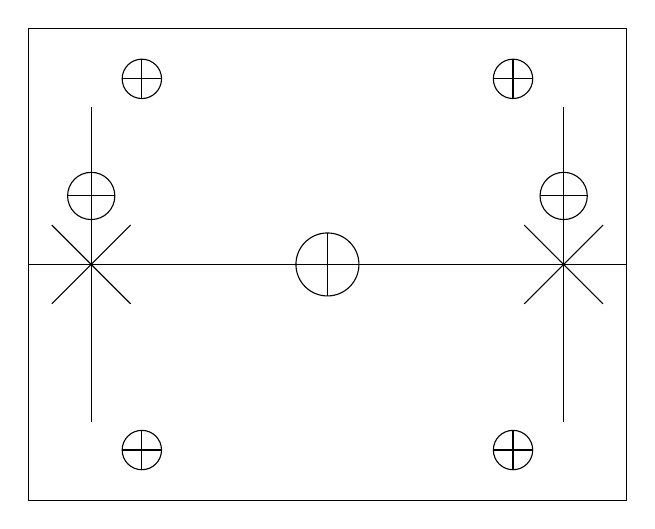
\begin{tikzpicture}[x=1mm, y=1mm]

% key points
\draw (-38, 0) -- (38, 0);
\draw (-30, -20) -- (-30, 20);
\draw (30, -20) -- (30, 20);
\draw (-35, -5) -- (-25, 5);
\draw (-35, 5) -- (-25, -5);
\draw (35, -5) -- (25, 5);
\draw (35, 5) -- (25, -5);

% proxxon mount holes
\hole{-30, 8.7}{3}
\hole{30, 8.7}{3}

% nema stepper shaft hole
\hole{0, 0}{4}

% nema stepper mount holes
\hole{-23.57, -23.57}{2.5}
\hole{23.57, -23.57}{2.5}
\hole{23.57, 23.57}{2.5}
\hole{-23.57, 23.57}{2.5}

\draw (-38, -30) rectangle (38, 30);
\end{tikzpicture}
\end{document}
